\documentclass[../draft.tex]{subfiles}

\begin{document}
    \chapter{Background}
    In this chapter we introduce the necessary background.

    \section{Static Data Flow Analysis}
    Muchnick \cite{Muchnick1997} defines data-flow analysis as follows:
    \begin{quote}
        Data-flow analysis provides global information about how a procedure (or a larger segment of a program) manipulates its data.
    \end{quote}
     
    In the field of compilers, there is a distinction between static and dynamic. Static generally refers to something that is decided at compile-time while dynamic refers to decisions taken at runtime \cite{Aho1986}. A common example is typing. In Java the type of a variable has to be declared before a value can be assigned to it while in Python the type of a variable is determined by the value assigned at runtime. Same distinction is also present for analyses. Dynamic analysis observes the run behavior of the program while static analysis works on a representation of the code. Both have different tradeoffs. Dynamic it is hard to achieve code coverage and static it is hard to not overapproximate the possible paths. 
    \begin{figure}[ht]
        \centering
        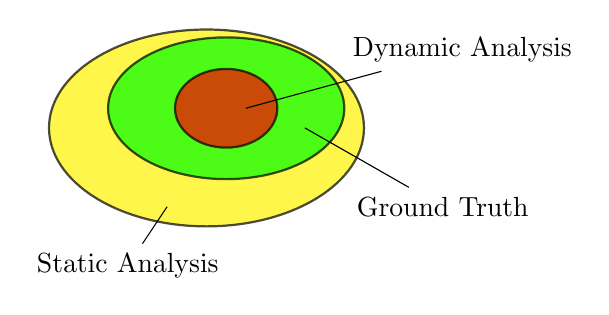
\begin{tikzpicture}
            \draw[fill=yellow, opacity=0.7, thick] (0,0) ellipse (2cm and 1.25cm);
            \draw[fill=green, opacity=0.7, thick] (0.25,0.25) ellipse (1.5cm and 0.9cm);
            \draw[fill=red, opacity=0.7, thick] (0.25, 0.25) ellipse (0.65cm and 0.5cm);


            \node (s) at (-1,-1.75) {Static Analysis};
            \draw (s) to (-0.5, -1);
            \node (d) at (3.25,1) {Dynamic Analysis};
            \draw (d) to (0.5, 0.25);
            \node (t) at (3, -1) {Ground Truth};
            \draw (t) to (1.25, 0);
        \end{tikzpicture}
        \caption{Data-flow Analysis Coverage}
    \end{figure}


    In taint analysis, a taint is a variable which contains interesting data. Sources provide data which is interesting and sinks leak data. A path from a source to a sink is leak.

    Explain key terms such as static, fact, taint, source, sink, leak, sensitivity.
    
    Static analyses are also categorized using sensitivities. These describe whether the analysis considers a certain aspect.
    First, there is flow-sensitivity. A flow-sensitive analysis can determine if a fact holds at a certain statement. Data-flow analyses are always flow-sensitive.
    Next up, context-sensitivity describes an interprocedural analysis which can distinguish the context of a called method, e.g. knows the original call site at a return.
    Object-sensitive analyses also distinguishes a fields between objects.
    Then there is also path-sensitivity. Basically, if an conditional branch is taken, the condition must hold and this knowledge is used by the analysis.

    \section{IFDS}
    \subsection{Original Definition}
    Interprocedural finite distributive subset (IFDS) problems are a special class of a data-flow analysis problem. All problems adhering to IFDS can be transformed into a graph-reachability problem and thus the solution is computable in polynomial time. It is context-sensitive and flow-sensitive by default.

    % graph
    IFDS operates on a so-called exploded supergraph. Every node in the exploded supergraph is a tuple $\langle s, d \rangle$ of a statement $s$ in the interprocedural control-flow graph and a dataflow fact $d$. The domain is typically the set of variables in the program. Edges between two nodes $\langle s, d \rangle$ and $\langle s', d' \rangle$ exist if $d$ propagated over $s$ yields $d'$ and $s'$ is a successor of $s$. This already ensures flow-sensitivity.

    % flow functions
    To propagate facts over statements, flow functions need to be defined. There are four types of flows:
    \begin{itemize}
        \item Call Flow: Edges from call statement into a method. Flow function maps the facts visible in the callee into it. 
        \item Return Flow: Edges returning from a method. Flow function maps the facts visible in the caller out of the method.
        \item Call To Return: Edges over a call statement. Flow function maps the facts not visible in the callee over the call statement.
        \item Normal Flow: Edges over every other statement. Often, this flow functions only handles assign statements.
    \end{itemize}
    The incoming set of facts is all predecessors' outgoing facts merged together using a merge operator $\sqcap$: 
    $$in(s) := \bigsqcap_{p \in Preds(s)} out(p)$$
    % introduce taints
    The domain also contains a zero fact and all nodes with $d=\textbf{0}$ are always reachable, thus the zero fact holds at every statement. As an example, in taint analysis the flow functions map zero facts at sources to a tainted variable. 

    % Context-Sensitive
    To ensure context-sensitivity, IFDS only visits valid paths. For this, a context-sensitive grammar is constructed which acts like a call stack to make sure there is no mismatch and the path is a valid execution path.
    The proposed tabulation algorithm to solve the reachable realizable path problem is a dynamic programming algorithm. Whenever a method was fully visited, a summary is saved and later on applied if the same input fact is observed. 

    % Fix point
    Eventually, there is no fact to propagate anymore and the analysis will stop. This is either because the facts were killed by the flow functions or already have been seen at the nodes and so reached a fixpoint.

    For all this to work, the problems which can be formulated in IFDS have to abide to restrictions which are also eponymous:

    \textbf{Distributive:} The flow function must be distributive over the merge operator. Formally, $f(x \sqcap y) = f(x) \sqcap f(y)$ must hold at any time. Informally speaking, it does not matter whether facts get merged before or after applying the flow functions. By defining the flow function signature as $f: \mathit{Fact} \rightarrow \mathit{Facts}$ with a single fact as an input but a set of facts as output, this property is trivially satisfied.

    \textbf{Finite:} Another restriction is that the set of dataflow facts has to be finite. Let's go by a counterexample of what IFDS is not capable of: Answering "Which value is stored in variable x at statement s?".
    Now the dataflow fact is a tuple of the variable together with the stored value $\langle x, v \rangle$. Assume $x$ is an integer of infinite precision for the domain to be infinite.
    $x$ is initialized to zero and passed into the method \code{foo()} multiple times. Recall the subset problem, then look at the summaries in \autoref{lst:ifdsfinite}. Clearly the purpose of creating summaries is lost because we never get to use the summary and also, there is no fixpoint for the ever growing subset to stop. Thus, the domain has to be finite and in practice, also small as the domain is cubic in the time-complexity $O(|E| \cdot |D|^3)$.
    \begin{figure}[ht]
        \centering
        \begin{subfigure}[b]{0.45\textwidth}
            \begin{lstlisting}[gobble=16]
                RealInteger foo(RealInteger x) {
                    return x + 42;
                }
            \end{lstlisting}
            \caption{Code}
        \end{subfigure}
        \begin{subfigure}[b]{0.45\textwidth}
            $$
                \begin{aligned}
                    \langle x, \phantom{0}0 \rangle &\rightarrow \langle x, \phantom{1}42 \rangle\\
                    \langle x, 42 \rangle &\rightarrow \langle x, \phantom{1}84 \rangle\\
                    \langle x, 84 \rangle &\rightarrow \langle x, 126 \rangle\\
                    &\dots
                \end{aligned}
            $$
            \caption{Summaries}
        \end{subfigure}
        \caption{Finitness example}
        \label{lst:ifdsfinite}
    \end{figure}

    \textbf{Subset:} IFDS also defines a underlying lattice on the powerset of the domain. The lattice ordering must be set inclusion. Following, the merge operator is set union.
  
    \subsection{Practical Extensions}
    The original definition is inefficient in practice. Among others, Naeem et al proposed practical extensions to the IFDS framework to perform better in practice \cite{Naeem2010}.

    Starting at the exploded supergraph, the original algorithm demands a fully built graph. Even in moderate programs the domain can get quite large and as the nodes in the exploded supergraph are the cross product of the domain and interprocedural call-graph nodes, it is infeasible to generate the full graph beforehand. Because there is no way to know before which part of the supergraph is actually needed, it is generated ad-hoc. This also removes the restriction on a small domain, now IFDS is also feasible if the encoutered subset of the domain is small enough \cite{Naeem2010}.
    The restrictions on the domain set can be loosened even more. Bodden suggests in-practice the domain can be infinite and only the observed facts must adhere to the ascending-chain condition over the flow functions when using the on-demand supergraph \cite{Bodden2012}.
    
    Also, it also ignores the type structure of the programming language. It can be used to kill facts due to impossible casts. Also, facts with the same variable but different types can be merged to one fact with the superclass as a type \cite{Naeem2010}.

    The original definition starts the IFDS algorithm at the entry point of the interprocedural call-graph. As described, whenever needed a fact is derived from the zero fact. If the methods where initial facts will be introduced are known a priori, the supergraph can be traversed without applying flow functions until such a method is found on the path. This optimization introduces unbalanced problems where a method return is found but no corresponding call site which can be solved by a small extension to the tabulation algorithm. This was first described by Lerch \cite{Lerch2015} and is also present in \textsc{FlowDroid} \cite{Arzt2017PhD}.     

    Because the merge operator is always set union, there is no need to wait for other predecessors to finish as a $A \subseteq A \cup B$ is always true. This allows the IFDS solver to skip the $in$-set construction and immediately propagate the outcoming facts, which is beneficial in a parallelized solver \cite{Arzt2017PhD} \todo{is this actually written anywhere?}.


    \section{Intermediate Representations}\label{s:jimple}
    Most compiler these days use intermediate representations (IRs). IRs are an equivalent representation of the source code but are much simpler and more regular and are typically not architecture dependent. They are often in an interchangeable format and can be saved as text to be able to use them by a variety of tools \cite{Thain2019}.
    This allows compilers to apply machine-independent optimizations to the code with neither worrying about complex expressions in the source code nor reimplementing the optimization for each architecture. 

    The Java Virtual Machine (JVM) also operates on an IR called Java bytecode. The JVM is mostly stack-based and so is the Java bytecode. In \autoref{lst:jvmstack} is an example of a simple code snippet translated to Java bytecode. Simple expressions such as \code{c = a + b} are translated into multiple statements and there is no fixed length of an expression in the bytecode. The analysis would also have to reconstruct the expressions ad-hoc. Furthermore, Java bytecode has over 200 possible instructions\footnote{\url{https://docs.oracle.com/javase/specs/jvms/se8/html/}} which need to be taken into account and only knows primitive types and references. Concluding, stack-based IRs are suitable for just-in-time interpretation but inconvenient for data flow analysis \cite{Valleerai2004}.

    \begin{figure}[ht]
        \centering
        \begin{subfigure}[b]{0.45\textwidth}
            \centering
            \begin{lstlisting}[gobble=16]
                int a = 21;
                int b = 21;
                int c = a + b;
            \end{lstlisting}
            \caption{Java code}
            \label{lst:jvmstack_a}
        \end{subfigure}
        \hfill
        \begin{subfigure}[b]{0.45\textwidth}
            \centering
            \begin{lstlisting}[gobble=16]
                bipush 21 // push 21
                istore_1  // store in register 1    
                bipush 21 // push 21
                istore_2 // store in register 2
                iload_1 // push a
                iload_2 // push b
                iadd // pop a & b and push a + b
                istore_3 // store in register 3
            \end{lstlisting}
            \caption{Java bytecode}
            \label{lst:jvmstack_b}
        \end{subfigure}
        \caption{Java bytecode example}
        \label{lst:jvmstack}
    \end{figure}

    A more convenient representation for static analysis are three-address codes. Each statement consists of up to three operands and is either an assigment or a control-flow statement. Such a representation is closer to the original source code while reducing the number of the possible combinations to a managable amount \cite{Aho1986}.

    Jimple is a three-address intermediate representation and can be constructed from the Java and Dalvik bytecode, the IR used for Android apps. It is a high-level representation and its syntax is close to Java. Complex expressions are split up into multiple statements, for example, there can be only one field reference per statement and arguments are always local variables. Jimple also reconstructs reference types \cite{Valleerai2004}. This greatly reduces the possible cases the data flow analysis needs consider and therefore is the IR of choice for FlowDroid \cite{Arzt2017PhD}. 
    The conversion to Jimple is provided by the underlying framework Soot. 

    \section{Soot}
    Soot is a 
    just short, but probably needs to be introduced before FlowDroid and especially before clinit rule
    \section{FlowDroid}    
\end{document}